\documentclass[border=6pt]{standalone}
\usepackage{tikz}
\usetikzlibrary{arrows.meta,calc,decorations.pathreplacing}
\begin{document}
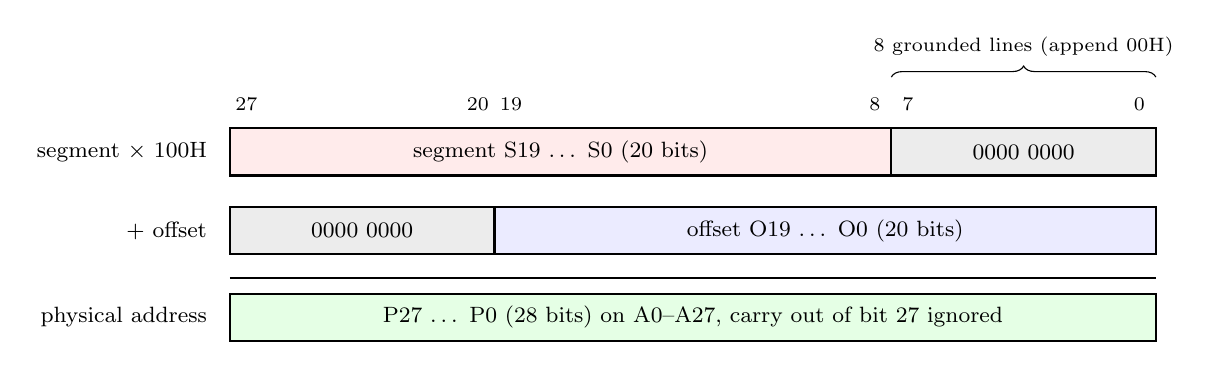
\begin{tikzpicture}[>=Stealth,font=\small,x=0.42cm,y=1cm,
 f/.style={draw,thick,minimum height=0.6cm,align=center,font=\footnotesize,inner sep=1pt}]
% 28 bit positions: x = 0 (bit 27) .. 28 (right edge, bit 0)
\foreach \b in {27,20,19,8,7,0} \node[font=\scriptsize] at (27-\b+0.5,0.6) {\b};
\node[anchor=east,font=\footnotesize] at (-0.4,0) {segment $\times$ 100H};
\draw[thick,fill=red!8] (0,-0.3) rectangle (20,0.3); \node[font=\footnotesize] at (10,0) {segment S19 \dots\ S0 (20 bits)};
\draw[thick,fill=gray!15] (20,-0.3) rectangle (28,0.3); \node[font=\footnotesize] at (24,0) {0000 0000};
\node[anchor=east,font=\footnotesize] at (-0.4,-1) {$+$ offset};
\draw[thick,fill=gray!15] (0,-1.3) rectangle (8,-0.7); \node[font=\footnotesize] at (4,-1) {0000 0000};
\draw[thick,fill=blue!8] (8,-1.3) rectangle (28,-0.7); \node[font=\footnotesize] at (18,-1) {offset O19 \dots\ O0 (20 bits)};
\draw[thick] (0,-1.6) -- (28,-1.6);
\node[anchor=east,font=\footnotesize] at (-0.4,-2.1) {physical address};
\draw[thick,fill=green!10] (0,-2.4) rectangle (28,-1.8); \node[font=\footnotesize] at (14,-2.1) {P27 \dots\ P0 (28 bits) on A0--A27, carry out of bit 27 ignored};
\draw[decorate,decoration={brace,amplitude=4pt}] (20,0.95) -- (28,0.95) node[midway,above=4pt,font=\scriptsize]{8 grounded lines (append 00H)};
\end{tikzpicture}
\end{document}
